\newpage
\criteria{Student Support Services}

\subcriteria{ The student intake policy, admission criteria, and admission procedures to the programme are shown to be clearly defined, communicated, published, and up-to-date.}
\noindent
{\bf การรับนักศึกษา}

	หลักสูตรกำหนดแผนการรับนักศึกษาปีละ 30 คน โดยรกำหนดนโยบายการรับนักศึกษา ช่องทางการรับเข้า คุณสมบัติของนักศึกษาที่จะรับเข้าศึกษา รวมถึงวิธีการคัดเลือกนักศึกษา และได้สื่อสารเผยแพร่ไปยังผู้มีส่วนได้ส่วนเสีย ได้แก่ นักเรียนชั้นมัธยมศึกษาปีที่ 6 ผู้ปกครอง และผู้ที่สนใจทั่วไป ผ่านเว็บไซต์ของมหาวิทยาลัยฯ คณะฯ และของสาขาวิชา รวมทั้ง Facebook ของคณะและสาขาวิชาฯ นอกจากนี้มีการออกประชาสัมพันธ์แนะแนวตามโรงเรียนที่เป็นกลุ่มเป้าหมายและโรงเรียนที่มีความร่วมมือทางวิชาการ (MOU)   กรอบการดำเนินงานเกี่ยวกับการรับนักศึกษาเป็นไปตามที่สำนักส่งเสริมวิชาการและงานทะเบียน (สวท.) เป็นผู้กำหนด เช่น ปฏิทินการรับสมัคร ระบบการสมัครทางระบบออนไลน์ การประกาศผล ฯลฯ ทั้งนี้ในแต่ละปีการศึกษากระบวนการรับนักศึกษามีขั้นตอนการดำเนินการดังนี้
	\begin{enumerate}
		\item งานทะเบียนฝ่ายวิชาการแจ้งให้หลักสูตรจัดทำข้อมูลรายละเอียดการรับสมัครนักศึกษาใหม่ เช่น จำนวนรับ คุณสมบัติผู้สมัคร วิธีการสอบคัดเลือก และคำแนะนำเกี่ยวกับหลักสูตร
		\item หลักสูตรจัดเตรียมข้อมูลเกณฑ์การรับ คุณสมบัติของนักศึกษา และแผนการรับนักศึกษา และส่งให้งานทะเบียนของคณะ 
		\item งานทะเบียนของคณะส่งข้อมูลเกณฑ์การรับ/คุณสมบัติของนักศึกษา แผนรับนักศึกษาไปยัง สวท. ของมหาวิทยาลัย เพื่อนำเข้าสู่การประชุมคณะกรรมการการบริหารวิชาการและวิจัย เพื่อพิจารณาอนุมัติและกำหนดไว้ในคู่มือการรับนักศึกษา
	\end{enumerate}
เมื่อได้รับกสนอนุมัติแผนรับแล้วหลักสูตรดำเนินการตามขั้นตอน วัน-เวลา การดำเนินการของมหาวิทยาลัยต่อไป\\

%%%%%%%%%%%%%%%%%%%%%%
\noindent{\bf เกณฑ์และขั้นตอนการรับเข้า}\\[0.5cm]
หลักสูตรกำหนดเกณฑ์การรับเข้าตามรอบการรับสมัครทั้งหมด 5 รอบ ได้แก่ โควตาMOU TCAS1 TCAS2 TCAS3 และ TCAS4
โดยเกณฑ์และคุณสมบัติของนักศึกษาที่จะรับเข้าในแต่ละรอบมีรายละเอียดดัง\underline{เอกสารหลักฐานระเบียบการรับสมัคร}
และแต่ละรอบมีขั้นตอนและกำหนดการสมัครดังรูป
\ref{Pic6.1-01}\\
\begin{figure}[h!]
	\begin{center}
		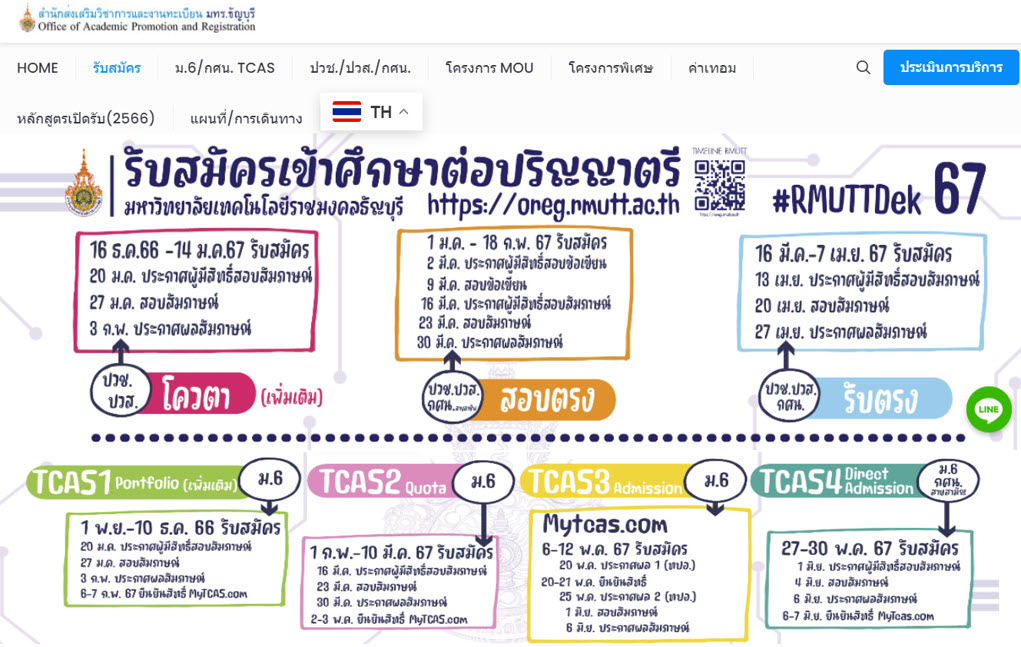
\includegraphics[width=0.65\textwidth]{Pic7.4-2.jpg}
		\end{center}
	\caption{รอบการรับสมัครและช่วงเวลาการรับสมัคร}
	\label{Pic6.1-01}
\end{figure}\\

%จากผลการดำเนินงานเกี่ยวกับการรับนักศึกษาในปีการศึกษา 2564–2566 ดังแสดงในตารางที่ \ref{table:6.1} พบว่า จำนวนนักศึกษาที่รายงานตัวมีแนวโน้มลดลงอย่างต่อเนื่อง เพื่อแก้ไขปัญหาดังกล่าว หลักสูตรจึงได้ดำเนินการวางแผนกลยุทธ์และปรับแนวทางการรับเข้าในปีการศึกษา 2567 ดังนี้
%\begin{enumerate}
%\item ปรับแผนการรับในแต่ละช่องทาง โดยเฉพาะช่องทาง TCAS 3 ซึ่งมีแนวโน้มตอบรับดีในปีก่อนหน้า โดยเพิ่มจำนวนแผนรับ ส่งผลให้มีนักศึกษารายงานตัวถึง 11 คนในปีการศึกษา 2567
%\item คงการเปิดรับผ่านช่องทางหลากหลาย ได้แก่ TCAS 1, TCAS 2, TCAS 4 และโควตา MOU เพื่อเพิ่มโอกาสและความหลากหลายในการเข้าถึงกลุ่มเป้าหมาย
%\item กระจายจำนวนแผนรับให้เหมาะสมกับประสิทธิภาพของแต่ละช่องทาง เช่น การลดแผนรับใน TCAS 1 และ TCAS 2 ซึ่งมีอัตราการรายงานตัวต่ำในปีก่อน
%\end{enumerate}
%
%จากการดำเนินกลยุทธ์ดังกล่าว ส่งผลให้จำนวนนักศึกษาที่รายงานตัวในปีการศึกษา 2567 เพิ่มขึ้นจาก 11 คนในปี 2566 เป็น 19 คน หรือคิดเป็นการเพิ่มขึ้นร้อยละ 72.7 ดังแสดงในตารางที่ \ref{table:6.1}

{\footnotesize
\begin{longtable}{ |c|c|c|c|c|c|c|c|c|}
\caption{ข้อมูลเปรียบเทียบแผนรับและจำนวนนักศึกษาที่รายงานตัวปีการศึกษา 2564-2567 }
\label{table:6.1}\\
 \hline
 \multicolumn{9}{|c|}{แผนรับ/รายงานตัว ปีการศึกษา 2564 – 2567} \\
 \hline
 ช่องทางการรับเข้า & \multicolumn{2}{c|}{2564} & \multicolumn{2}{c|}{2565} & \multicolumn{2}{c|}{2566} & \multicolumn{2}{c|}{2567} \\
 \cline{2-9}
  & แผนรับ & รายงานตัว & แผนรับ & รายงานตัว & แผนรับ & รายงานตัว & แผนรับ & รายงานตัว \\
 \hline
  TCAS1 & 10 & 6 & 15 & 5 &  15 &   1  & 10 & 3\\
 \hline
   TCAS2& 10 & 3 & 8 & 2 &  7 &   0 & 4 & 2\\
 \hline
   TCAS3& 4 & 5 & 6 & 5 &  7 &  7  & 15 & 11\\
 \hline
   TCAS4 & 2 & 2 & 1 & 2 & 1  & 2   & 1 & 2 \\
 \hline
 โควตา MOU  & 4 & 18 & - &  9 & -  & 1   &  - & 1\\
 \hline
  รวม  & 30  & 34 & 30 &  23 & 30  &  11  & 30 & 19\\
 \hline
\end{longtable}
}




จากผลการดำเนินงานด้านการรับนักศึกษาในช่วงปีการศึกษา 2564–2566 (ตารางที่ \ref{table:6.1}) พบว่าจำนวนนักศึกษาที่รายงานตัวลดลงอย่างต่อเนื่อง ซึ่งสะท้อนถึงความท้าทายในการสรรหาผู้เรียนเข้าสู่หลักสูตรวิทยาศาสตรบัณฑิต สาขาวิชาคณิตศาสตร์ เพื่อแก้ไขปัญหาดังกล่าวและตอบสนองต่อคำแนะนำของผู้เชี่ยวชาญ หลักสูตรจึงได้วางแผนและดำเนินกลยุทธ์การรับเข้าใหม่ในปีการศึกษา 2567 โดยยึดตามข้อมูลเชิงประจักษ์จากผลสำรวจช่องทางการรับรู้ข้อมูลหลักสูตรของนักศึกษาที่เข้าศึกษาในปีการศึกษา 2566 (ตารางที่ \ref{table:6.2})
%%%%%%%%%%%%%%%%%%%%%%%%%%%%
%%%%%%%%%%%%%%%%%%%%%%%%%

\begin{longtable}{ |>{\raggedright}p{6cm}|c|}
\caption{การรับรู้จากสื่อการประชาสัมพันธ์ของนักศึกษาที่รับเข้าในปีการศึกษา 2566}
\label{table:6.2}\\ 
\hline
\multicolumn{1}{|c|}{{\bf ช่องทางการประชาสัมพันธ์}}     & \multicolumn{1}{c|}{\textbf{ร้อยละของผู้ตอบแบบสอบถาม }}   
\\
\hline
\endfirsthead

\caption[]{(ต่อ) การรับรู้จากสื่อการประชาสัมพันธ์ของนักศึกษาที่รับเข้าในปีการศึกษา 2566}
\\
\hline
\multicolumn{1}{|c|}{{\bf ช่องทางการประชาสัมพันธ์}}     & \multicolumn{1}{c|}{\textbf{ร้อยละของผู้ตอบแบบสอบถาม }}   
\\
\hline
\endhead
1. เพื่อน  &   11.54\\ 
\hline
2. ครูแนะแนว &   25 \\ 
\hline
3. แนะแนวสัญจร &   11.54 \\ 
\hline
4. เว็บไซค์คณะวิทยาศาสตร์และเทคโนโลยี  &  38.46  \\ 
\hline
5. เพจคณะวิทยาศาสตร์และเทคโนโลยี    &   1.92 \\ 
\hline
6. เพจสาขาวิชาคณิตศาสตร์ &  5.77  \\ 
\hline
7. อื่นๆ  & 5.77  \\ 
\hline
\end{longtable}




ผลสำรวจชี้ว่าช่องทางการประชาสัมพันธ์ที่มีอิทธิพลสูงสุด ได้แก่ เว็บไซต์ของคณะวิทยาศาสตร์และเทคโนโลยี (ร้อยละ 38.46) รองลงมาคือครูแนะแนว (ร้อยละ 25) และกิจกรรมแนะแนวสัญจร (ร้อยละ 11.54) หลักสูตรได้นำข้อมูลดังกล่าวมาใช้ในการกำหนดแนวทางกลยุทธ์ ดังนี้:
\begin{enumerate}
	\item พัฒนาเว็บไซต์ของคณะฯ ให้เป็นช่องทางหลักในการนำเสนอข้อมูลหลักสูตร ข่าวสาร และกิจกรรม เพื่อเสริมสร้างภาพลักษณ์และความน่าสนใจต่อผู้สมัคร
	\item เสริมสร้างความร่วมมือกับครูแนะแนว เพื่อขยายเครือข่ายการประชาสัมพันธ์ไปยังโรงเรียนในพื้นที่เป้าหมาย
	\item เพิ่มความถี่และคุณภาพของกิจกรรมแนะแนวสัญจร โดยเน้นการมีปฏิสัมพันธ์กับนักเรียนเป้าหมายโดยตรง
	\item ปรับแผนการรับในแต่ละช่องทาง โดยเฉพาะการเพิ่มจำนวนรับในรอบ TCAS3 ซึ่งมีแนวโน้มตอบรับดีในปีก่อน
	\item คงการรับผ่านช่องทางที่หลากหลาย ได้แก่ TCAS1 TCAS2 TCAS4 และโควตา MOU เพื่อเปิดโอกาสให้กลุ่มเป้าหมายที่หลากหลายสามารถเข้าถึงหลักสูตรได้
	\item กระจายจำนวนแผนรับตามประสิทธิภาพของแต่ละช่องทาง โดยลดจำนวนแผนรับใน TCAS1 และ TCAS2 ที่มีอัตราการรายงานตัวต่ำในปีก่อนหน้า
\end{enumerate}
ผลจากการดำเนินกลยุทธ์ข้างต้น ส่งผลให้จำนวนนักศึกษาที่รายงานตัวในปีการศึกษา 2567 เพิ่มขึ้นจาก 11 คนในปี 2566 เป็น 19 คน หรือเพิ่มขึ้นร้อยละ 72.7 (ตารางที่ \ref{table:6.1}) แสดงให้เห็นถึงความสำเร็จในการประยุกต์ใช้ข้อมูลเชิงประจักษ์และการตัดสินใจเชิงกลยุทธ์ในการบริหารจัดการการรับนักศึกษาอย่างมีประสิทธิภาพ




     
นอกกจากนี้ ในปีการศึกษา 2567 หลักสูตรได้สำรวจเกี่ยวกับช่องทางการประชาสัมพันธ์ของนักศึกษาที่รับเข้าแสดงดังตาราง \ref{table:6.3}
\begin{longtable}{ |>{\raggedright}p{6cm}|c|}
\caption{การรับรู้จากสื่อการประชาสัมพันธ์ของนักศึกษาที่รับเข้าในปีการศึกษา 2567}
\label{table:6.3}\\
\hline
\multicolumn{1}{|c|}{{\bf ช่องทางการประชาสัมพันธ์}}     & \multicolumn{1}{c|}{\textbf{ร้อยละของผู้ตอบแบบสอบถาม }}   
\\
\hline
\endfirsthead

\caption[]{(ต่อ) การรับรู้จากสื่อการประชาสัมพันธ์ของนักศึกษาที่รับเข้าในปีการศึกษา 2567}
\\
\hline
\multicolumn{1}{|c|}{{\bf ช่องทางการประชาสัมพันธ์}}     & \multicolumn{1}{c|}{\textbf{ร้อยละของผู้ตอบแบบสอบถาม }}   
\\
\hline
\endhead
1. เพื่อน  &   3 \\ 
\hline
2. ครูแนะแนว &   14  \\ 
\hline
3. แนะแนวสัญจร &   14  \\ 
\hline
4. เว็บไซค์คณะวิทยาศาสตร์และเทคโนโลยี  &  41   \\ 
\hline
5. เพจคณะวิทยาศาสตร์และเทคโนโลยี    &    10 \\ 
\hline
6. เพจสาขาวิชาคณิตศาสตร์ &   10  \\ 
\hline
7. อื่นๆ  &  7  \\ 
\hline
\end{longtable}

จากผลการสำรวจนักศึกษาที่เข้าศึกษาในปีการศึกษา 2567 (ตารางที่ \ref{table:6.3}) พบว่า ช่องทางการรับรู้ข้อมูลหลักสูตรที่มีอิทธิพลสูงสุดคือ เว็บไซต์คณะวิทยาศาสตร์และเทคโนโลยี มทร.ธัญบุรี (ร้อยละ 41) รองลงมาคือ ครูแนะแนว และกิจกรรมแนะแนวสัญจร (ร้อยละ 14 เท่ากัน) ส่วนเพจของคณะฯ และของสาขาวิชาอยู่ในระดับปานกลาง (ร้อยละ 10 ต่อช่องทาง) ข้อมูลนี้สะท้อนว่าเว็บไซต์คณะฯ เป็นช่องทางสื่อสารที่มีประสิทธิภาพสูงสุด รองลงมาคือเครือข่ายบุคลากรแนะแนวและกิจกรรมนอกสถานที่ ขณะที่โซเชียลมีเดียยังคงมีบทบาทสำคัญ โดยเฉพาะในกลุ่มนักเรียนที่ใช้งานแพลตฟอร์มออนไลน์เป็นประจำ
    
 
 \begin{doclist}
 	\docitem{เว็บไซต์/ Facebook การประชาสัมพันธ์}
 	\docitem{ระเบียบการรับสมัครนักศึกษาปีการศึกษา 2567}
 \end{doclist}

%%%%%%%%%%%%%% 6.2 %%%%%%%%%%%%%%%

\subcriteria{Both short-term and long-term planning of academic and non-academic support services are shown to be carried out to ensure sufficiency and quality of support services for teaching, research, and community service.}
%%%%%%%%%%%%%%%%%%%%%%%%%%%%%%%%%%%%%%%%%%%%%%%%%
หลักสูตรมีแผนการจัดโครงการ/กิจกรรมให้กับนักศึกษา ทั้งแผนระยะสั้นและแผนระยะยาว โดยเน้นการส่งเสริมและพัฒนานักศึกษาด้านวิชาการและด้านที่ไม่ใช่วิชาการใน 3 ด้าน ดังนี้
\begin{enumerate}
	\item โครงการ/กิจกรรมทางด้านวิชาการและวิชาชีพ 
	\item โครงการ/กิจกรรมเตรียมความพร้อมก่อนเข้าสู่การทำงานที่สอดคล้องกับทักษะการเรียนรู้ในศตวรรษที่ 21
	\item โครงการ/กิจกรรมเพื่อพัฒนาทักษะทางสังคม
\end{enumerate}
%%%%%%%%%%%%%%%%%%%%%%%%%%%%%%%%%%%%%%%%%%%%%%%%%%%%%%5
\textbf{แผนระยะยาวราย 4 ปี (ปีการศึกษา 2567-2570)} มีรายละเอียดดังนี้
\begin{longtable}{|c >{\raggedright}p{9cm}|c|c|c|c|}
	\hline
	&\multicolumn{1}{c|}{\multirow{2}{*}{\textbf{โครงการ/กิจกรรม}}}&\multicolumn{4}{c|}{\textbf{ปีการศึกษา}}\\
	\cline{3-6}
	&&2567 &2568 &2569 & 2570 \\\hline
\multicolumn{6}{|l|}{\textbf{โครงการ/กิจกรรมที่สนับสนุนด้านวิชาการ}}\\\hline
1.&โครงการถ่ายทอดประสบการณ์จริงสู่การฝึกประสบการณ์วิชาชีพ สาขาวิชาคณิตศาสตร์& \checkmark  & \checkmark & \checkmark  & \checkmark \\\hline
2.&โครงการการพัฒนาศักยภาพด้านการเรียนรู้เชิงลึกสำหรับการแก้ปัญหาในศตวรรษที่ 21 & \checkmark  & \checkmark & \checkmark  & \checkmark \\\hline
3.&โครงการพัฒนาทักษะกระบวนการคิดและการเรียนรู้ในการส่งเสริมความเป็นนวัตกรของนักศึกษาสาขาวิชาคณิตศาสตร์ & \checkmark  & \checkmark & \checkmark  & \checkmark \\\hline
\multicolumn{6}{|l|}{\textbf{โครงการ/กิจกรรมที่สนับสนุนด้านที่ไม่ใช่วิชาการ}}\\\hline
4.&กิจกรรมเตรียมความพร้อมเข้าสู่รั้วมหาวิทยาลัยและปฐมนิเทศนักศึกษาใหม่สาขาวิชาคณิตศาสตร์ %(กิจกรรม First Date Mathematics ปฐมนิเทศนักศึกษาสาขาวิชาคณิตศาสตร์ประยุกต์ รุ่นที่ 23 AM67111)
	 & \checkmark  & \checkmark & \checkmark  & \checkmark \\\hline
5.&	กิจกรรมสานสัมพันธ์ น้อง-พี่ สาขาวิชาคณิตศาสตร์  & \checkmark  & \checkmark & \checkmark  & \checkmark \\\hline
6.&	กิจกรรมแสดงความยินดีกับพี่บัณฑิต สาขาวิชาคณิตศาสตร์ & \checkmark  & \checkmark & \checkmark  & \checkmark \\\hline
7.&	กิจกรรมปัจฉิมนักศึกษาสาขาวิชาคณิตศาสตร์  & \checkmark  & \checkmark & \checkmark  & \checkmark \\\hline
\end{longtable}	
\textbf{แผนระยะสั้น} หลักสูตรกำหนดแผนการจัดโครงการ/กิจกรรมเพิ่มเติมจากแผนระยะยาวในปีการศึกษา 2567  ดังนี้ 
\begin{longtable}{|c >{\raggedright}p{8.7cm}|c|c|}
	\hline
	&\centering\textbf{โครงการ/กิจกรรม}&\textbf{สนับสนุนด้าน}&\textbf{สนับสนุนด้าน}\\
&&\textbf{วิชาการ}&\textbf{ที่ไม่ใช่วิชาการ}\\\hline
	1.&ส่งเสริมให้นักศึกษาเข้าร่วมประกวด/นำเสนอผลงานในงานประชุมวิชาการด้านคณิตศาสตร์/คณิตศาสตร์ประยุกต์& \checkmark & \\\hline
%	1. ร่วมนำเสนอผลงานแบบบรรยาย ในงาน การประชุมวิชาการระดับปริญญาตรีด้านคณิตศาสตร์ประยุกต์ ครั้งที่ 13 (UAMC2025) &    & \checkmark &    &  \\\hline
%	2. โครงการบริการวิชาการศิษย์เก่า สาขาวิชาคณิตศาสตร์ คณะวิทยาศาสตร์และเทคโนโลยี  &   &   & \checkmark  &   \\\hline
	2.&ส่งเสริมให้นักศึกษาร่วมแสดงนิทรรศการในกิจกรรม Open house  &  \checkmark  &   \\\hline
	3.&ส่งเสริมการจัดกิจกรรมด้านจิตอาสา &    & \checkmark \\\hline
\end{longtable}	
%%%%%%%%%%%%%%%%%%%%%%%%%%%
\newpage
ในปีการศึกษา 2567 หลักสูตรได้ดำเนินการจัดโครงการ/กิจกรรมตามแผนที่กำหนดทั้งแผนระยะสั้นและแผนระยะยาว ซึ่งมีรายละเอียดดังนี้\\
%%%%%%%%%%%%%%%%%%%%%%%%%%%%%%%%%%
\textbf{แผนงานระยะยาว}
\begin{longtable}{|>{\raggedright}p{0.3\textwidth}|>{\centering}p{0.18\textwidth}|>{\raggedright}p{0.32\textwidth}|>{\centering\arraybackslash}p{0.13\textwidth}|}
	\hline
	\centering{\textbf{โครงการ/กิจกรรม}}   & \textbf{วันที่ดำเนินการ} &  \centering{\textbf{ผลการดำเนินงาน}} & \textbf{ผู้รับผิดชอบ}  \\ \hline
	\endfirsthead
	\hline
	\centering{\textbf{โครงการ/กิจกรรม}}   & \textbf{วันที่ดำเนินการ} &  \centering{\textbf{ผลการดำเนินงาน}} & \textbf{ผู้รับผิดชอบ}  \\ \hline
	\endhead
	1.	กิจกรรมเตรียมความพร้อมเข้าสู่รั้วมหาวิทยาลัยและปฐมนิเทศนักศึกษาใหม่สาขาวิชาคณิตศาสตร์ (กิจกรรม First Date Mathematics ปฐมนิเทศนักศึกษาสาขาวิชาคณิตศาสตร์ประยุกต์ รุ่นที่ 23 AM67111)  & 9 สิงหาคม 2567 
	& หลักสูตรจัดกิจกรรม First Date Mathematics ปฐมนิเทศนักศึกษาสาขาวิชาคณิตศาสตร์ประยุกต์ รุ่นที่ 23 AM67111 โดยให้ความรู้เกี่ยวกับหลักสูตร ระบบงานทะเบียน ตารางเรียน  เพื่อให้นักศึกษาใหม่ได้ปรับตัวด้านการวางแผนการศึกษาในระดับมหาลัยวิทยาลัย ทั้งด้านวิชาการและการใช้ชีวิต รวมไปถึงให้ความรู้แก่นักศึกษาในเรื่องการเรียนสำหรับรายวิชาที่มีการเขียนโปรแกรม เพื่อให้นักศึกษามีความพร้อมทางด้านการใช้ชีวิตในรั้วมหาวิทยาลัย มีความพร้อมทางด้านการเรียน มีความมุ่งมั่นที่จะเรียน สามารถศึกษาในระดับอุดมศึกษาได้ประสบผลสำเร็จ และสำเร็จการศึกษาได้ตามระยะเวลาที่หลักสูตรกำหนด & อาจารย์ที่ปรึกษาชั้นปีที่ 1 \\ \hline
	2.โครงการถ่ายทอดประสบการณ์จริงสู่การฝึกประสบการณ์วิชาชีพ: สาขาวิชาคณิตศาสตร์  & 6 มีนาคม 2568 
	&  หลักสูตรจัดโครงการถ่ายทอดประสบการณ์จริงสู่การฝึกประสบการณ์วิชาชีพ โดยได้รับเกียรติจาก คุณพิกุลทอง บุญภิละ (ศิษย์เก่าสาขาวิชาคณิตศาสตร์) จาก บริษัทเอไอเอ จำกัด มาเป็นวิทยากรบรรยายในหัวข้อ ``การเรียนรู้จากประสบการณ์จริงจากการฝึกประสบการณ์วิชาชีพทางด้านคณิตศาสตร์ประกันภัย และการสร้างตัวแบบทางคณิตศาสตร์''
	& หลักสูตร \\ \hline
	3.	โครงการปัจฉิมนิเทศ ปีการศึกษา 2567 ``โครงการเตรียมความพร้อมสู่สถานประกอบการ'' สําหรับนักศึกษาชั้นปีที่ 4  & 7 มีนาคม 2567 & หลักสูตรจัดโครงการเตรียมความพร้อมสู่สถานประกอบการสําหรับนักศึกษาชั้นปีที่ 4 โดยได้รับเกียรติจาก นายสิรภพ ศิลาสุวรรณ (ศิษย์เก่าสาขาวิชาคณิตศาสตร์) บริษัทวิริยะประกันภัย จำกัด (มหาชน) มาเป็นวิทยากรบรรยายในหัวข้อ ``คณิตศาสตร์กับงานประกันภัย''  &  อาจารย์ที่ปรึกษาชั้นปีที่ 4\\ \hline
	4.	กิจกรรมสานสัมพันธ์ น้อง-พี่ สาขาวิชาคณิตศาสตร์   
	& 19 กุมภาพันธ์ 2568 & หลักสูตรได้จัดกิจกรรมสานสัมพันธ์ น้อง-พี่ สาขาวิชาคณิตศาสตร์ เมื่อวันที่ 19 กุมภาพันธ์ 2568 ซึ่งกิจรรมนี้มีวัตถุประสงค์เพื่อเป็นการกระชับความสัมพันธ์อันดีระหว่างอาจารย์ และนักศึกษา รุ่นพี่-รุ่นน้อง ในสาขาวิชาฯ พร้อมทั้งจัดพิธีมอบทุนการศึกษาให้กับนักศึกษาที่มีผลการเรียนดี และขาดแคลทุนทรัพย์ &  หลักสูตร \\ \hline
	5.	กิจกรรมแสดงความยินดีกับพี่บัณฑิตสาขาวิชาคณิตศาสตร์   &  20 พฤศจิกายน 2567 
	& หลักสูตรได้จัดกิจกรรมแสดงความยินดีกับพี่บัณฑิต เมื่อวันที่ 20 พฤศจิกายน 2567 โดยมีวัตถุประสงค์เพื่อ แสดงความยินดีกับบัณฑิตของสาขาวิชา ส่งเสริมให้นักศึกษาในสาขาวิชามีความสัมพันธ์ที่ดีต่อกัน ส่งเสริมให้นักศึกษาใหม่ได้รู้จักพี่บัณฑิต อีกทั้งยังเห็นแนวทางในการประกอบอาชีพและเกิดเจตคติที่ดีต่อการเรียนในหลักสูตรฯ & หลักสูตร \\ \hline
	6.	โครงการการพัฒนาศักยภาพด้านการเรียนรู้เชิงลึกสำหรับการแก้ปัญหาในศตวรรษที่ 21   & 5-6 เมษายน 2568 
	& หลักสูตรได้จัดโครงการพัฒนาศักยภาพด้านการเรียนรู้เชิงลึกสำหรับการแก้ปัญหาในศตวรรษที่ 21 โดยมุ่งให้นักศึกษาสามารถใช้ TensorFlow ในการสร้างแบบจำลองการเรียนรู้เชิงลึก และประยุกต์ใช้ในการแก้ปัญหาจริงที่รับความสนใจในปัจจุบัน  นอกจากนี้ นักศึกษาที่เข้าร่วมโครงการจำนวน 10 คน ยังได้รับใบประกาศนียบัตรด้านการเรียนรู้เชิงลึกจากองค์กรหรือหน่วยงานที่ได้รับการยอมรับในระดับนานาชาติด้านปัญญาประดิษฐ์อีกด้วย &  หลักสูตรฯ \\ \hline
	7.	โครงการพัฒนาทักษะกระบวนการคิดและการเรียนรู้ในการส่งเสริมความเป็นนวัตกรของนักศึกษาสาขาวิชาคณิตศาสตร์  & 11, 23 กุมภาพันธ์ 2568 
	& หลักสูตรได้จัดโครงการพัฒนาทักษะกระบวนการคิดและการเรียนรู้ในการส่งเสริมความเป็นนวัตกรของนักศึกษาสาขาวิชาคณิตศาสตร์
	โดยนำนักศึกษาไปศึกษาดูงานที่บริษัทบ้านปู จำกัด (มหาชน) เมื่อวันที่ 11 กุมภาพันธ์ 2568 และเชิญวิทยากรจากหน่วยงานภายนอกมาบรรยายเมื่อวันที่ 23 กุมภาพันธ์ 2568 ณ คณะวิทยาศาสตร์และเทคโนโลยี ทำให้นักศึกษาได้รับความรู้ ความเข้าใจ และแนวคิดเกี่ยวกับการทำงานด้านการจัดการศึกษา การเงินและธนาคาร การวิเคราะห์ข้อมูล และเทคโนโลยีดิจิทัล และสามารถนำความรู้จากห้องเรียนไปประยุกต์ใช้ในสถานการณ์จริงได้อย่างเหมาะสม& หลักสูตร\\\hline
\end{longtable}


\noindent
\textbf{แผนงานระยะสั้น}

\begin{longtable}{|>{\raggedright}p{0.3\textwidth}|>{\centering}p{0.18\textwidth}|>{\raggedright}p{0.32\textwidth}|>{\centering\arraybackslash}p{0.13\textwidth}|}
	\hline
	\centering{\textbf{โครงการ/กิจกรรม}}   & \textbf{วันที่ดำเนินการ} &  \centering{\textbf{ผลการดำเนินงาน}} & \textbf{ผู้รับผิดชอบ}  \\
	 \hline
	 \endhead
	1. ร่วมนำเสนอผลงานแบบบรรยาย ในงาน การประชุมวิชาการระดับปริญญาตรีด้านคณิตศาสตร์ประยุกต์ ครั้งที่ 13 (UAMC2025)	   & 30 มีนาคม 2568  & หลักสูตรฯได้สนับสนุนให้นักศึกษาจากสาขาวิชาคณิตศาสตร์  ได้แก่ นายหัสชัย ครองแถว นายณัฐพนธ์ ปรีชานุวัฒน์และนายพงศกร งานภักดีสกุล ร่วมนำเสนอผลงานแบบบรรยาย ในงาน การประชุมวิชาการระดับปริญญาตรีด้านคณิตศาสตร์ประยุกต์ ครั้งที่ 13 (UAMC2025)	  ซึ่งจัดขึ้นเมื่อวันอาทิตย์ที่ 30 มีนาคม 2568 ณ สำนักการเรียนรู้ตลอดชีวิตพระจอมเกล้าเจ้าคุณทหารลาดกระบัง สถาบันเทคโนโลยีพระจอมเกล้าเจ้าคุณทหารลาดกระบัง  โดยนักศึกษาทั้งสามได้รับรางวัลเหรียญทองแดงจากการนำเสนอผลงานวิจัยแบบบรรยาย ในหัวข้อ ``การวางแผนการจัดส่งสินค้าหลายวันจากหลายคลังสินค้า''
	&  หลักสูตรฯ  \\ \hline
	2. โครงการอบรมเชิงปฏิบัติการ ``การสร้างสื่อการเรียนการสอนเพื่อพัฒนาศักยภาพของครู'' &  29 มีนาคม พ.ศ. 2568  & สาขาวิชาคณิตศาสตร์ คณะวิทยาศาสตร์และเทคโนโลยี มหาวิทยาลัย มหาวิทยาลัยเทคโนโลยีราชมงคลธัญบุรี จัดโครงการอบรมเชิงปฏิบัติการ ``การสร้างสื่อการเรียนการสอนเพื่อพัฒนาศักยภาพของครู'' สำหรับศิษย์เก่าสาขาวิชาคณิตศาสตร์และนักศึกษาจากสาขาวิชาคณิตศาสตร์   ในวันที่ 29 มีนาคม พ.ศ. 2568  ณ ห้องปฏิบัติการคอมพิวเตอร์ คณะวิทยาศาสตร์และเทคโนโลยี  โดยผู้เข้าร่วมได้พัฒนาทักษะและศักยภาพของครูในการสร้างสื่อการเรียนการสอนที่มีประสิทธิภาพและเหมาะสมกับบริบทของผู้เรียนในศตวรรษที่ 21 & หลักสูตรฯ \\ \hline
	3. ร่วมจัดบูทในงาน Open house RMUTT 2025 & 17-18 มกราคม 2568  & หลักสูตรฯได้สนับสนุนให้นักศึกษาจากสาขาวิชาคณิตศาสตร์  ร่วมจัดบูทกิจกรรมในงาน Open house RMUTT 2025 เพื่อส่งเสริมให้นักศึกษามีส่วนร่วมในการเผยแพร่และประชาสัมพันธ์หลักสูตร ตลอดจนแสดงศักยภาพทางวิชาการผ่านการจัดกิจกรรมในงาน Open House RMUTT 2025 &  หลักสูตรฯ\\ \hline
	4. กิจกรรมจิตอาสาพัฒนาสาขาวิชาคณิตศาสตร์ &   &   &  \\ \hline
\end{longtable}
%%%%%%%%%%%%%%%%%%%%%%%%%%%%%%%%%%%%%%%%%%%%

นอกจากนี้ในปีการศึกษา 2567 ยังมีการดำเนินโครงการ/กิจกรรมที่สนับสนุนด้านวิชาการและที่ไม่ใช่วิชาการตามแผนรายปีของคณะวิทยาศาสตร์และเทคโนโลยี ซึ่งมีรายละเอียดดังนี้
\begin{longtable}{|p{0.2cm} >{\raggedright}p{9cm}|c|c|}
	\caption{โครงการ/กิจกรรมที่สนับสนุนด้านวิชาการและไม่ใช่วิชาการปีการศึกษา 2567}
	\label{table:PDF-2567}\\
	\hline
	\multicolumn{2}{|c|}{\multirow{2}{*}{\textbf{โครงการ/กิจกรรม (ผู้รับผิดชอบดำเนินการ)}}} &  \textbf{สนับสนุนด้าน} & \textbf{สนับสนุนด้าน} \\
	&&  \textbf{ วิชาการ} & \textbf{ที่ไม่ใช่วิชาการ} \\
	\hline
	\endfirsthead
		\caption{(ต่อ) โครงการ/กิจกรรมที่สนับสนุนด้านวิชาการและไม่ใช่วิชาการปีการศึกษา 2567}\\
	\hline
	\multicolumn{2}{|c|}{\multirow{2}{*}{\textbf{โครงการ/กิจกรรม (ผู้รับผิดชอบดำเนินการ)}}} &  \textbf{สนับสนุนด้าน} & \textbf{สนับสนุนด้าน} \\
	&&  \textbf{ วิชาการ} & \textbf{ที่ไม่ใช่วิชาการ} \\
	\hline
	\endhead
	1.&กิจกรรมปฐมนิเทศนักศึกษาใหม่ สานสัมพันธ์น้องพี่คณะวิทยาศาสตร์และเทคโนโลยีประจำปีการศึกษา 2567 (ฝ่ายพัฒนานักศึกษา) & & \checkmark \\ \hline
	2.&โครงการไหว้ครู คณะวิทยาศาสตร์และเทคโนโลยี ประจำปีการศึกษา 2567 (ฝ่ายพัฒนานักศึกษา) & & \checkmark \\\hline
	3.&กิจกรรมปัจฉิมนิเทศนักศึกษาสหกิจศึกษา ประจำปีการศึกษา 2567 (ฝ่ายวิชาการ) & \checkmark & \\ \hline
	4.&กิจกรรมเตรียมความพร้อมการฝึกประสบการณ์วิชาชีพ ประจำภาคการศึกษาที่ 2/2567 (ฝ่ายวิชาการ) & \checkmark & \\ \hline
	5.&โครงการค้นหาตัวแทนนักกีฬาคณะวิทยาศาสตร์และเทคโนโลยีเพื่อเข้าร่วมการแข่งขัน บัวน้ำเงินเกมส์ ครั้งที่ 30 (ฝ่ายพัฒนานักศึกษา) & & \checkmark \\ \hline
	6.&โครงการเตรียมความพร้อมสู่สถานประกอบการ ภาคการศึกษา 2/2567 (ฝ่ายพัฒนานักศึกษา)  & \checkmark &  \\ \hline
	7.&โครงการ คิด ลอง ดู เป็นผู้ประกอบการ คณะวิทยาศาสตร์และเทคโนโลยี (ฝ่ายพัฒนานักศึกษา) & \checkmark &   \\ \hline
	8.&โครงการต้นกล้าความดี พัฒนาวิถีชุมชน (ฝ่ายพัฒนานักศึกษา) & \checkmark &   \\ \hline
	9.&โครงการค้นหาทูตกิจกรรม Atomic Constellation Boys \& Girls 2024 (ฝ่ายพัฒนานักศึกษา) & & \checkmark \\ \hline
	10.&โครงการสัมมนาพัฒนาศักยภาพผู้นำนักศึกษาคณะวิทยาศาสตร์และเทคโนโลยี ปีการศึกษา 2567 (ฝ่ายพัฒนานักศึกษา) & & \checkmark \\
	\hline
\end{longtable}
%%%%%%%%%%%%%%%%%%%%%%%%%%%%


%\newpage
%หลักสูตรมีการบริการสนับสนุนทางด้านวิชาการและที่ไม่ใช่ทางวิชาการ เพื่อพัฒนาทักษะของนักศึกษาโดยมีการดำเนินการกิจกรรม ตามแผนงานที่จัดทำเพื่อพัฒนาประสบการณ์ ทางวิชาการและวิชาชีพแก่ นักศึกษาโดยมีกิจกรรม ดังนี้\\
%
%\noindent
%\textbf{แผนงานระยะสั้น}
%\begin{longtable}{ |>{\raggedright}p{3cm}|p{10.5cm}|} 
%\hline
%\centering{\textbf{กิจกรรม}}   &\multicolumn{1}{c|}{\textbf{รายละเอียด}} \\ \hline
%\endhead
%1. กิจกรรมบรรยายพิเศษ ในหัวข้อ “ ” โดย     &  
%\\ 
%\hline
%2. กิจกรรมบรรยายพิเศษ ในหัวข้อ " " โดย   &    
%   \\ 
%\hline
%\end{longtable}
%
%\newpage
%\noindent
%\textbf{แผนงานระยะยาว}
%\begin{longtable}{ |>{\raggedright}p{3cm}|p{10.5cm}|} 
%\hline
%\centering{\textbf{กิจกรรม}}   & \multicolumn{1}{c|}{\textbf{รายละเอียด}} \\ \hline
%1. กิจกรรม First Date Mathematics ปฐมนิเทศนักศึกษาสาขาวิชาคณิตศาสตร์ประยุกต์ รุ่นที่ 23 AM67111   
%& หลักสูตรได้มอบหมายให้อาจารย์ปรึกษาชั้นปีที่ 1 เป็นผู้รับผิดชอบโครงการ โดยมีการให้ความรู้เกี่ยวกับหลักสูตร ระบบงานทะเบียน ตารางเรียน     
%เพื่อให้นักศึกษาใหม่ได้ปรับตัวด้านการวางแผนการศึกษาในระดับมหาลัยวิทยาลัย ทั้งด้านวิชาการและการใช้ชีวิต รวมไปถึงให้ความรู้แก่นักศึกษาในเรื่องการเรียนสำหรับรายวิชาที่มีการเขียนโปรแกรม เพื่อให้นักศึกษามีความพร้อมทางด้านการใช้ชีวิตในรั้วมหาวิทยาลัย มีความพร้อมทางด้านการเรียน มีความมุ่งมั่นที่จะเรียน สามารถศึกษาในระดับอุดมศึกษาได้ประสบผลสำเร็จ และสำเร็จการศึกษาได้ตามระยะเวลาที่หลักสูตรกำหนด
%\\ 
%\hline
%2. กิจกรรมสานสัมพันธ์ น้อง-พี่ สาขาวิชาคณิตศาสตร์   
%&   หลักสูตรได้จัดกิจกรรมสานสัมพันธ์ น้อง-พี่ สาขาวิชาคณิตศาสตร์ เมื่อวันที่ 19 กุมภาพันธ์ 2568 ซึ่งกิจรรมนี้มีวัตถุประสงค์เพื่อเป็นการกระชับความสัมพันธ์อันดีระหว่างอาจารย์ และนักศึกษา รุ่นพี่-รุ่นน้อง ในสาขาวิชาฯ พร้อมทั้งจัดพิธีมอบทุนการศึกษาให้กับนักศึกษาที่มีผลการเรียนดี และขาดแคลทุนทรัพย์
%   \\ 
%\hline
%3. กิจกรรมแสดงความยินดีกับพี่บัณฑิต  
%& หลักสูตรได้จัดกิจกรรมแสดงความยินดีกับพี่บัณฑิต เมื่อวันที่ 20 พฤศจิกายน 2567 โดยมีวัตถุประสงค์เพื่อ แสดงความยินดีกับบัณฑิตของสาขาวิชา ส่งเสริมให้นักศึกษาในสาขาวิชามีความสัมพันธ์ที่ดีต่อกัน ส่งเสริมให้นักศึกษาใหม่ได้รู้จักพี่บัณฑิต อีกทั้งยังเห็นแนวทางในการประกอบอาชีพและเกิดเจตคติที่ดีต่อการเรียนในหลักสูตรฯ
%   \\ 
%\hline
%4. กิจกรรมปัจฉิมนักศึกษาสาขาวิชาคณิตศาสตร์ รหัส 64
%& หลักสูตรได้จัดกิจกรรมปัจฉิมนักศึกษาสาขาวิชาคณิตศาสตร์ รหัส 64 เมื่อวันที่ 7 มีนาคม 2568 เพื่อเตรียมความพร้อมก่อนสำเร็จการศึกษา เสริมสร้างความตระหนักรู้เกี่ยวกับเส้นทางอาชีพในอนาคต การปรับตัวสู่โลกการทำงาน และการเป็นศิษย์เก่าที่มีคุณภาพ
% \\ 
%\hline
%4. โครงการการพัฒนาศักยภาพด้านการเรียนรู้เชิงลึกสำหรับการแก้ปัญหาในศตวรรษที่ 21
%& หลักสูตรได้จัดโครงการการพัฒนาศักยภาพด้านการเรียนรู้เชิงลึกสำหรับการแก้ปัญหาในศตวรรษที่ 21 เพื่อ{\color{red}วัตถุประสงค์....}
%ระหว่างวันที่ 5-6 เมษายน 2568 ณ คณะวิทยาศาสตร์และเทคโนโลยี มหาวิทยาลัยเทคโนโลยีราชมงคลธัญบุรี 
%\\ 
%\hline
%5. โครงการพัฒนาทักษะกระบวนการคิดและการเรียนรู้ในการส่งเสริมความเป็นนวัตกรของนักศึกษาสาขาวิชาคณิตศาสตร์ 
%& หลักสูตรได้จัดโครงการพัฒนาทักษะกระบวนการคิดและการเรียนรู้ในการส่งเสริมความเป็นนวัตกรของนักศึกษาสาขาวิชาคณิตศาสตร์ เพื่อเพิ่มสมรรถนะสู่การประกอบอาชีพ จัดขึ้นในวันที่ 23 กุมภาพันธ์ 2568 ห้อง ST1-906 คณะวิทยาศาสตร์และเทคโนโลยี
%\\ 
%\hline
%\end{longtable}
%
%\newpage
%นอกจากนี้ หลักสูตรได้มีการบริการสนับสนุนทางด้านวิชาการและที่ไม่ใช่ทางวิชาการ โดยได้ดำเนินการผ่านทางคณะวิทยาศาสตร์และเทคโนโลยีดังตารางต่อไปนี้
%\begin{longtable}{ |>{\raggedright}p{4.5cm}|p{9cm}|} 
%\hline
%\centering{\textbf{กิจกรรม}}   & \multicolumn{1}{c|}{\textbf{รายละเอียด}} \\
% \hline
% \endhead
%1. กิจกรรมเตรียมความพร้อมการฝึกประสบการณ์วิชาชีพ ประจำภาคการศึกษาที่ 2/2567
%& งานสหกิจศึกษา ฝ่ายวิชาการ คณะวิทยาศาสตร์และเทคโนโลยี จัดกิจกรรมเตรียมความพร้อมการฝึกประสบการณ์วิชาชีพ ประจำภาคการศึกษาที่ 2/2567 โดยได้รับเกียรติจากวิทยากร บรรยาย และกิจกรรม WORKSHOP หัวข้อ แนวคิดการเป็นผู้ประกอบการและการสร้างสรรค์นวัตกรรมเชิงพาณิชย์สำหรับนักศึกษาฝึกประสบการณ์วิชาชีพ โดย คุณปาพจน์ ตันสุวรรณ ผู้เชี่ยวชาญอิสระด้านการพัฒนานวัตกรรม จัดขึ้นในวันที่ 20 กุมภาพันธ์ 2568 ในรูปแบบออนไลน์
%\\ 
%\hline
%2. โครงการถ่ายทอดประสบการณ์จริงสู่การฝึกประสบการณ์วิชาชีพ: สาขาวิชาคณิตศาสตร์
%& งานสหกิจศึกษา ฝ่ายวิชาการ คณะวิทยาศาสตร์และเทคโนโลยี มทร.ธัญบุรี จัดโครงการถ่ายทอดประสบการณ์จริงสู่การฝึกประสบการณ์วิชาชีพ: สาขาวิชาคณิตศาสตร์ โดยได้รับเกียรติจาก คุณพิกุลทอง บุญภิละ (ศิษย์เก่าสาขาวิชาคณิตศาสตร์) จาก บริษัท เอไอเอ จำกัด มาเป็นวิทยากรบรรยายในหัวข้อ การเรียนรู้จากประสบการณ์จริงจากการฝึกประสบการณ์วิชาชีพทางด้านคณิตศาสตร์ประกันภัย และการสร้างตัวแบบทางคณิตศาสตร์  ในวันที่ 6 มีนาคม 2568 ณ ห้อง ST1-906 คณะวิทยาศาสตร์และเทคโนโลยี
%\\ 
%\hline
%3. โครงการ Science game 2024 
%& 
%\\ 
%\hline
%4. โครงการเตรียมความพร้อมสู่สถานประกอบการ ภาคการศึกษา 2/2567 
%& 
%   \\ 
%\hline
%5. โครงการ คิด ลอง ดู เป็นผู้ประกอบการ คณะวิทยาศาสตร์และเทคโนโลยี 
%& ผศ.ดร.นิพัทธ์ จงสวัสดิ์ คณบดีคณะวิทยาศาสตร์และเทคโนโลยี เป็นประธานเปิดโครงการคิด ลอง ดู เป็นผู้ประกอบการ คณะวิทยาศาสตร์และเทคโนโลยี เพื่อสร้างความรู้และความเข้าใจ ตลอดจนกระตุ้นให้นักศึกษาเกิดแรงบันดาลใจในการเป็นผู้ประกอบการด้านวิทยาศาสตร์ประยุกต์ โดยได้รับเกียรติจากวิทยากรผู้ทรงคุณวุฒิภายนอก ได้แก่ คุณชลวัชร เรืองรุจิระ (CEO บริษัท สตรัท โปรเฟสชั่น จำกัด) คุณอรรถพร ดุษฎี (ผู้บริหารจากบริษัท CTC จำกัด) คุณรฉัตร โรจนพิชยกุล (CEO บริษัท เอ็มครีเอทีฟ จำกัด/ศิษย์เก่า) และคุณชนัญธิดา ทะพลี (CEO บริษัท แอทฟลาวเวอร์ จำกัด/ศิษย์เก่า) ในวันที่ 14 มีนาคม 2567 ณ ห้องสงค์ธนาพิทักษ์ มทร.ธัญบุรี
%   \\ 
% \hline
%6. โครงการปฐมนิเทศนักศึกษาใหม่สานสัมพันธ์พี่น้องคณะวิทยาศาสตร์และเทคโนโลยี ประจำปีการศึกษา 2567 
%& ฝ่ายพัฒนานักศึกษา คณะวิทยาศาสตร์และเทคโนโลยี จัดโครงการปฐมนิเทศนักศึกษาใหม่สานสัมพันธ์พี่น้องคณะวิทยาศาสตร์และเทคโนโลยี ประจำปีการศึกษา 2567 เพื่อให้นักศึกษาใหม่มีความเข้าใจบทบาท หน้าที่และสามารถนำมาใช้เป็นแนวทางการใช้ชีวิตในรั้วมหาวิทยาลัย และปรับตัวเข้ากับสังคมระดับอุดมศึกษา นักศึกษาใหม่ได้รับข้อมูลข่าวสารที่เป็นประโยชน์และสามารถนำไปประยุกต์ใช้ในชีวิตประจำวัน นักศึกษาใหม่รู้จักสถานที่ภายในรั้วมหาวิทยาลัย คณะ สาขาต่าง ๆ อาจารย์และเจ้าหน้าที่ นักศึกษาใหม่ได้ทำความรู้จักและสร้างความสัมพันธ์ รวมถึงการอยู่ร่วมกันด้วยความสามัคคีกับรุ่นพี่ในคณะวิทยาศาสตร์และเทคโนโลยี ในวันที่ 20 มิถุนายน 2567 ณ คณะวิทยาศาสตร์และเทคโนโลยี มหาวิทยาลัยเทคโนโลยีราชมงคลธัญบุรี
%\\
%\hline
%7. โครงการไหว้ครู คณะวิทยาศาสตร์และเทคโนโลยี ประจำปีการศึกษา 2567 
%&  ผศ.ดร.นิพัทธ์ จงสวัสดิ์ คณบดีคณะวิทยาศาสตร์และเทคโนโลยี เป็นประธานในพิธีไหว้ครู คณะวิทยาศาสตร์และเทคโนโลยี ประจำปีการศึกษา 2567 ในวันที่ 18 กรกฎาคม 2567 ณ ห้องประชุมสงค์ธนาพิทักษ์ มหาวิทยาลัยเทคโนโลยีราชมงคลธัญบุรี
%   \\ 
%\hline
%8. โครงการต้นกล้าความดี พัฒนาวิถีชุมชน  
%& 
%ฝ่ายพัฒนานักศึกษา คณะวิทยาศาสตร์และเทคโนโลยี จัดโครงการต้นกล้าความดี พัฒนาวิถีชุมชน โดยได้รับเกียรติจาก ผศ.ดร.มรกต พุทธกาล รองคณบดีฝ่ายพัฒนานักศึกษา เป็นประธานเปิดโครงการ ในวันที่ 22 สิงหาคม 2567 ณ ห้องประชุมนลินวิทย์ คณะวิทยาศาสตร์และเทคโนโลยี
% \\ 
%\hline
%9. โครงการ SciTech Freshy Day 
%& 
%\\ 
%\hline
%10. โครงการสัมมนาพัฒนาศักยภาพผู้นํานักศึกษาคณะวิทยาศาสตร์และเทคโนโลยี ปีการศึกษา 2567
%& 
%\\ 
%\hline
%11. โครงการค้นหาตัวแทนนักกีฬาคณะวิทยาศาสตร์และเทคโนโลยีเข้าร่วมการแข่งขันบัวน้ําเงินเกมส์ครั้งที่ 30 
%& 
%\\ 
%\hline
%12. โครงการค้นหาทูตกิจกรรม Atomic Constellation Boys \& Girls 2024
%& 
%\\ 
%\hline
%13. กิจกรรมประกวดผู้อัญเชิญตราและสุดยอดพิธีกร 
%& 
%\\ 
%\hline
%14. โครงการจิตอาสาทําความสะอาดคณะวิทยาสาสตร์และเทคโนโลยี 
%& 
%\\ 
%\hline
%\end{longtable}



\begin{doclist}
%	\docitem{เว็บไซต์ www.oreg.rmutt.ac.th}
	\docitem{ภาพ/รายงานการดำเนินกิจกรรม/โครงการของสาขาวิชา}
	\docitem{ภาพ/รายงานการดำเนินกิจกรรม/โครงการของฝ่ายพัฒนานักศึกษา/ฝ่ายวิชาการ}
\end{doclist}

%%%%%%%%%%% 6.3 %%%%%%%%%%%%%%%%%%%%%%
\subcriteria{An adequate system is shown to exist for student progress, academic performance, and workload monitoring. Student progress, academic performance, and workload are shown to be systematically recorded and monitored. Feedback to students and corrective actions are made where necessary.}


หลักสูตรมีระบบติดตามความก้าวหน้าของนักศึกษา ตรวจสอบผลการศึกษา และภาระการเรียนของนักศึกษา ดังนี้
 \begin{enumerate}
 	\item  หลักสูตรมีระบบการติดตามความก้าวหน้าทางด้านผลการเรียน รายวิชาที่ยังเรียนไม่ครบในหลักสูตร การทดลองคำนวณเกรด โดยนักศึกษาสามารถตรวจสอบข้อมูลได้จากระบบงานทะเบียนของสำนักส่งเสริมวิชาการและงานทะเบียน (www.oreg.rmutt.ac.th) 
 	\item หลักสูตรมีระบบอาจารยที่ปรึกษา โดยแต่งตั้งอาจารย์ที่ปรึกษารายชั้นปี เพื่อวางแผนเกี่ยวกับการดูแลการให้คำปรึกษา โดย
 \begin{enumerate}[label=(\arabic*),leftmargin=0.8cm, labelsep=2mm]
 	\item ก่อนเปิดภาคการศึกษาอาจารย์ที่ปรึกษาให้คำแนะนำเกี่ยวกับการลงทะเบียนเรียน
	\item สัปดาห์แรกของภาคการศึกษา อาจารย์ที่ปรึกษานัดพบนักศึกษาเพื่อพูดคุยและกำหนดวัน-เวลาในการให้คำปรึกษา (Homeroom) 
	\item อาจารย์ที่ปรึกษามีการให้ข้อมูลย้อนกลับแก่นักศึกษาในกรณีที่นักศึกษามีปัญหาทางด้านผลการเรียน และให้คำแนะนำปรึกษาเป็นรายบุคคล โดย
	\begin{itemize}
		\item กรณีที่นักศึกษามีผลการเรียนเฉลี่ยสะสม (GPAX) ไม่ถึง 2.00 จะมีการล็อคระบบการลงทะเบียนของนักศึกษาเพื่อให้นักศึกษามาพบเพื่อให้คำแนะนำและร่วมวางแผนการลงทะเบียนเรียนในแต่ละภาคการศึกษา  
		\item ให้นักศึกษาเข้าพบอาจารย์ที่ปรึกษาเดือนละ 2 ครั้ง เพื่อให้อาจารย์ที่ปรึกษาสามารถติดตามความก้าวหน้าทางการเรียน ให้คำแนะนำและแก้ปัญหาได้ทันเวลา
		\item ให้นักศึกษารายงานผลคะแนนสอบกลางภาคให้อาจารย์ที่ปรึกษาทราบ กรณีที่มีรายวิชาที่นักศึกษาได้คะแนนสอบกลางภาคน้อย อาจารย์ที่ปรึกษาจะแนะนำให้นักศึกษาถอนรายวิชาดังกล่าว 
	\end{itemize}
	\item อาจารย์ที่ปรึกษากำกับติดตามและประเมินความเสี่ยงที่อาจเกิดขึ้นในด้านต่าง ๆ นอกเหนือจากด้านผลการเรียนและให้คำแนะนำปรึกษา
	\item เมื่อสิ้นสุดภาคการศึกษา ให้อาจารย์ที่ปรึกษาทำสรุปผลการดำเนินงานเสนอต่ออาจารย์ผู้รับผิดชอบหลักสูตร
	\item เมื่อสิ้นสุดปีการศึกษา หลักสูตรให้นักศึกษาทุกชั้นปีประเมินความพึงพอใจต่อระบบอาจารย์ที่ปรึกษาซึ่งมี ผลการประเมินแสดงดังตาราง\\[0.25cm] 
		\begin{tabular}{ |l|c|} 
		%\caption{ผลการประเมินความพึงพอใจของนักศึกษาต่อระบบอาจารย์ที่ปรึกษา}
		%\label{Table:T}
		\hline
		\centering{\textbf{ความพึงพอใจที่มีต่อระบบอาจารย์ที่ปรึกษา}} & \textbf{คะแนนเฉลี่ยความพึงพอใจ} \\
		\hline
		1. ด้านการให้คำปรึกษาเชิงวิชาการ &   4.51\\ 
		\hline
		2. ด้านการให้คำปรึกษาหรือแจ้งกิจกรรมด้านพัฒนานักศึกษา &   4.47 \\ 
		\hline
		3. ด้านรูปแบบ/เวลาการให้คำปรึกษา &  4.39 \\ 
		\hline
		\textbf{ความพึงพอใจในภาพรวม} & \textbf{4.47}  \\ 
		\hline
	\end{tabular}
		จากตารางพบว่า นักศึกษามีความพึงพอใจในภาพรวมอยู่ในระดับพึงพอใจมากที่สุด (คะแนนเฉลี่ย 4.47 จากคะแนนเต็ม 5)
	\item หลักสูตรรวบรวมและสรุปผลการประเมินความพึงพอใจของนักศึกษาและนำผลการประเมินที่ได้ไปปรับปรุงแก้ไขในส่วนที่เกี่ยวข้อง
	\end{enumerate}

%\item ระบบกิจกรรมนักศึกษา: มหาวิทยาลัยมีระบบบันทึกชั่วโมงกิจกรรมที่นักศึกษาได้ทำไปแล้ว ซึ่งสามารถตรวจสอบได้ตามจำนวนชั่วโมงที่มหาวิทยาลัยกาหนดจากเว็บไซต์ https://activity.rmutt.ac.th/login.php ในส่วนของอาจารย์ที่ปรึกษาจะคอยช่วยกำกับดูแลนักศึกษาเป็นรายบุคคลเพื่อให้นักศึกษามีชั่วโมงกิจกรรมครบตามที่มหาวิทยาลัยกำหนด
%\begin{figure}[h!]
%    \centering
%    {\includegraphics[width=8.5cm]{6.3-1.png}}
%    \caption{ระบบติดตามชั่วโมงกิจกรรมของนักศึกษา}
%    \label{fig6.3-1}
%\end{figure}
\item หลักสูตรมีการติดตามภาระงาน (workload) ของนักศึกษาเพื่อไม่ให้มีภาระงานมากเกินไป  โดยมอบหมายให้อาจารย์ที่ปรึกษากำกับและติดตามภาระงาน (workload) ของนักศึกษา ซึ่งมีกระบวนการดังนี้
 		\begin{enumerate}[label=(\arabic*),leftmargin=0.8cm, labelsep=2mm]
		\item อาจารย์ที่ปรึกษานัดพบนักศึกษา (Homeroom) อย่างน้อยเดือนละ 1 ครั้ง และสอบถามนักศึกษาเรื่องการสั่งงาน/การบ้านของแต่ละวิชา
		\item อาจารย์ที่ปรึกษาพูดคุยกับอาจารย์ผู้สอนแต่ละวิชาเพื่อหาแนวทางในการลดภาระงาน (workload) ของนักศึกษา ยกตัวอย่าง เช่น  
		\begin{itemize}
			\item รายวิชา 09-114-204 การเขียนโปรแกรมคอมพิวเตอร์ทางคณิตศาสตร์ และรายวิชา 09-114-223 การสร้างแบบจำลองทางคณิตศาสตร์เบื้อง ซึ่งมีเนื้อหาบางส่วนที่เกี่ยวข้องกัน  อาจารย์ผู้สอนทั้งสองรายวิชาได้ร่วมกันออกแบบกิจกรรมการเรียนรู้ โดยมอบหมายงานกลุ่มให้นักศึกษาเพียง 1 ชิ้นงาน ที่สามารถใช้เป็นคะแนนในทั้งสองวิชา
			\item รายวิชา 09-115-304 ทักะการนำเสนอผลงานทางด้านคณิตศาสตร์ และรายวิชา  09-115-401 สัมมนาทางคณิตศาสตร์ประยุกต์ โดยในรายวิชาทักษะการนำเสนอผลงานทางด้านคณิตศาสตร์  อาจารย์ผู้สอนให้นักศึกษานำบทความวิจัยที่นำเสนอในรายวิชาสัมมนาทางคณิตศาสตร์ประยุกต์มาฝึกนำเสนอหน้าชั้นเรียนและเปิดโอกาสให้เพื่อนซักถามหน้าชั้นเรียน รวมทั้งให้แสดงความคิดเห็น
		\end{itemize}
		\end{enumerate}

\end{enumerate}
\begin{doclist}
	\docitem{เว็บไซต์ www.oreg.rmutt.ac.th }
	\docitem{แบบบันทึกการเข้ากิจกรรมให้คำปรึกษา (Homeroom)}
\end{doclist}

%%%%%%%%%%% 6.4 %%%%%%%%%%%%%%%%%%%%%%

\subcriteria{Co-curricular activities, student competition, and other student support services are shown to be available to improve learning experience and employability.}

  
\begin{enumerate}
	\item  หลักสูตรได้จัดกิจกรรมเสริมหลักสูตรเพื่อเพิ่มประสบการณ์ ความรู้และทักษะให้กับนักศึกษา ครอบคลุมทั้งด้านวิชาการและทักษะความสามารถในการทำงาน พร้อมทั้งส่งเสริมการเรียนรู้ตลอดชีวิต โดยมีการกิจกรรมเสริมหลักสูตร ดังนี้ \\
\begin{tabular}{ |>{\raggedright}p{6cm}|c|c| } 
\hline
\centering{\textbf{ชื่อโครงการ/กิจกรรม}}   & \centering{\textbf{วัน/เดือน/ปี}} &  \textbf{จำนวนผู้เข้าร่วม} \\ \hline
กิจกรรม First Date Mathematics ปฐมนิเทศนักศึกษาสาขาวิชาคณิตศาสตร์ประยุกต์ รุ่นที่ 23 AM67111 &  9 สิงหาคม 2567  & 29   \\
\hline
กิจกรรมสานสัมพันธ์ น้อง-พี่ สาขาวิชาคณิตศาสตร์ &  19 กุมภาพันธ์ 2568    &  66 \\
\hline
กิจกรรมแสดงความยินดีกับพี่บัณฑิต  &  20 พฤศจิกายน 2567 & 66  \\
\hline
กิจกรรมปัจฉิมนักศึกษาสาขาวิชาคณิตศาสตร์ รหัส 64 & 7 มีนาคม 2568  &  38 \\
\hline
\end{tabular}

\item  หลักสูตรส่งเสริมสนับสนุนให้นักศึกษาเข้าร่วมประกวด/แข่งขัน ดังนี้ 
 \begin{enumerate}[label=(\arabic*),leftmargin=0.8cm, labelsep=2mm]

 \item  
หลักสูตรส่งนักศึกษาเข้าร่วมการประกวดผลงานสหกิจศึกษา-วิทยาศาสตร์ดีเด่น ระดับคณะฯ ประจำภาคการศึกษาที่ 1/2567 จัดขึ้นในวันที่ 13 ธันวาคม 2567  ณ   อาคารเฉลิมพระเกียรติ 6 รอบ พระชนมพรรษา จำนวน 2 ประเภท ดังตารางต่อไปนี้\\[0.25cm] 
  \begin{tabular}{|>{\raggedright}p{3cm}|>{\raggedright}p{4cm}|p{4.2cm}|}
   \hline
   \centering{\textbf{ประเภท}} & \centering{\textbf{ผลงาน}} & \textbf{ชื่อ-นามสกุล นักศึกษา} \\
    \hline
  โครงงานสหกิจศึกษา ด้านวิทยาศาสตร์และเทคโนโลยีดีเด่น  &  โครงงานโปรแกรมสร้างแท็กหรือตราสินค้า
 &  นายหัสชัย ครองแถว \par 
นายพงศกร\;งานภักดีสกุล \\ \hline
  โครงงานสหกิจศึกษา ด้านนวัตกรรมดีเด่น  & การจำแนกพารามิเตอร์การทดสอบแบ็คเอนด์ของ HDDs โดยใช้แบบจำลองการเรียนรู้ของเครื่อง  &  นางสาววรรณษา เหรียญทอง \par 
นายปฏิภาณ สมวงศ์   \\ \hline
    \end{tabular}
   \item  หลักสูตรส่งเสริมและสนับสนุนให้นักศึกษาชั้นปีที่ 4 เข้าร่วมการประชุมวิชาการระดับปริญญาตรีด้านคณิตศาสตร์ประยุกต์ ครั้งที่ 13 (UAMC2025) ซึ่งจัดขึ้นในวันอาทิตย์ที่ 30 มีนาคม พ.ศ. 2568 ณ สำนักการเรียนรู้ตลอดชีวิตพระจอมเกล้าเจ้าคุณทหารลาดกระบัง สถาบันเทคโนโลยีพระจอมเกล้าเจ้าคุณทหารลาดกระบัง โดยมีนักศึกษาสาขาวิชาคณิตศาสตร์ ได้แก่
\begin{enumerate}[label=\arabic*),leftmargin=1.5cm]
\item นายหัสชัย ครองแถว
\item นายณัฐพนธ์ ปรีชานุวัฒน์
\item นายพงศกร งานภักดีสกุล
\end{enumerate}
เข้าร่วมการนำเสนอผลงานแบบบรรยาย และได้รับ รางวัลระดับเหรียญทองแดง จากผลงานเรื่อง การวางแผนการจัดส่งสินค้าหลายวันจากหลายคลังสินค้า
\end{enumerate}
    
     
    
\item หลักสูตรส่งเสริมให้นักศึกษาเข้ารับการทดสอบสมรรถนะจากองค์กรภายนอกในรายวิชา 09114339 วิทยาการข้อมูลสำหรับนักคณิตศาสตร์ อาจารย์ผู้สอนสนับสนุนให้นักศึกษาสอบวัดระดับความสามารถด้านการเรียนรู้เชิงลึกจากองค์กรหรือหน่วยงานที่ได้รับการยอมรับในระดับสากล ผลปรากฏว่านักศึกษาทุกคนที่ลงทะเบียนเรียนวิชานี้ จำนวน  18 คน ได้รับใบประกาศนียบัตรอย่างน้อยหนึ่งใบจาก IBM คิดเป็นร้อยละ 100
\item หลักสูตรส่งนักศึกษาเข้าร่วมกิจกรรมของทางคณะวิทยาศาสตร์และเทคโนโลยี เพื่อเสริมสร้างประสบการณ์ ความรู้และทักษะให้กับนักศึกษา ครอบคลุมทั้งทางด้านวิชาการและทักษะความสามารถในการทำงาน ดังตาราง \ref{table:PDF-2567} (Criterion 6.2)\\ 
\end{enumerate}		
\begin{doclist}
	\docitem{ภาพกิจกรรม/รายงานการดำเนินกิจกรรม/โครงการของสาขาวิชา }
	\docitem{ใบประกาศนียบัตร }
\end{doclist}


%%%%%%%% 6.5 %%%%%%%%%%%%%%%%%%%%%%%
\subcriteria{The competences of the support staff rendering student services are shown to be identified for recruitment and deployment. These competences are shown to be evaluated to ensure their continued relevance to stakeholders needs. Roles and relationships are shown to be well-defined to ensure smooth delivery of the services.}
\noindent\textbf{การกำหนดสมรรถนะและความสามารถของเจ้าหน้าที่สายสนับสนุน} 

เป็นไปตามกรอบของคณะและมหาวิทยาลัย  โดยคณะมีการจัดทำคำบรรยายลักษณะงาน  (Job Description) คุณสมบัติเฉพาะตำแหน่ง  (Job Specification)  ที่ชัดเจน เกี่ยวกับความสามารถในการให้บริการนักศึกษา มีการกำหนดวิธีการประเมินผลที่มีความ
ชัดเจน เพื่อให้มั่นใจว่า สามารถให้บริการได้อย่างมีประสิทธิภาพแก่ผู้มารับบริการ \\

\noindent\textbf{ระบบการสรรหาบุคลากรสายสนับสนุน}

ในการคัดเลือกบุคลากรสายสนับสนุน คณะฯ ยึดถือตามระเบียบของมหาวิทยาลัยเป็นหลัก และพิจารณาผู้ที่มีคุณสมบัติเฉพาะตำแหน่งเหมาะสมกับงานที่จะได้รับมอบหมาย มีการจัดทำประกาศรับสมัครซึ่งได้กำหนดคุณสมบัติประจำตำแหน่ง บทบาทหน้าที่ ลักษณะงานที่รับผิดชอบ เงินเดือน สวัสดิการ ฯลฯ มีการสื่อสารผ่านทางเว็บไซต์ของคณะและมหาวิทยาลัย\\

\noindent\textbf{การประเมินสมรรถนะของบุคลากรสายสนับสนุน}

ในการประเมินสมรรถนะของบุคลากรสายสนับสนุนจะเป็นการประเมินเพื่อเลื่อนขั้นเงินเดือน  ซึ่งมีการประเมินปีละ 2 ครั้ง (ครั้งที่ 1 คือ 1 ตุลาคม - 31 มีนาคม และ ครั้งที่ 2 คือ 1 เมษายน - 30 กันยายน)  โดยมีคะแนนประเมินจาก 2 ส่วนประกอบคือ 
\begin{enumerate}
\item การประเมินผลสัมฤทธิ์ของบุคลากรสายสนับสนุนในสถาบันอุดมศึกษา มหาวิทยาลัยเทคโนโลยีราชมงคลธัญบุรี คิดเป็นสัดส่วนคะแนน 70\% โดยแบ่งออกเป็น
\begin{enumerate}[label=(\arabic*),leftmargin=0.8cm, labelsep=2mm]
\item ด้านคุณภาพและปริมาณงาน
\item ด้านความรู้ความสามารถในการปฏิบัติงาน
\item การสร้างผลงานคู่มือปฏิบัติงานหรืองานวิจัย R2R
\item การเข้าร่วมงานและงานมอบหมายอื่น ๆ
\end{enumerate}
\item ประเมินสมรรถนะหลักของบุคลากรสายวิชาการที่กำหนดโดยมหาวิทยาลัย 6 ด้าน คิดเป็นสัดส่วนคะแนน 30\% ได้แก่
\begin{enumerate}[label=(\arabic*),leftmargin=0.8cm, labelsep=2mm]
\item รักองค์กรและหน้าที่ มีจิตสำนึก ในการเป็นเจ้าของ เห็นคุณค่าองค์กร มุ่งมั่นการทำงานในหน้าที่อย่างเป็นระบบ มีวินัยและคุณธรรมพัฒนาตนเอง และองค์กรไปสู่เป้าหมายอย่างต่อเนื่อง
\item พัฒนาตนเองเรียนรู้วิทยาการใหม่ๆเพื่อพัฒนาและเพิ่มศักยภาพในการทำงานที่มีประสิทธิภาพและสอดคล้องต่อการเปลี่ยนแปลง มีความรู้ ความเชี่ยวชาญ
\item เป็นมืออาชีพ มีความรู้ ความเชี่ยวชาญ ในการปฏิบัติงาน และเชื่อมโยง แก้ไขปัญหาในการทำงานได้ อย่างเหมาะสมตามจรรยาบรรณวิชาชีพ
\item สื่อสารอย่างสร้างสรรค์ การถ่ายทอดข้อมูลข่าวสารโดยใช้สื่อต่างๆ มีการแลกเปลี่ยนความคิดเห็น และสร้างความเข้าใจร่วมกันในการทำงาน อย่างมีประสิทธิภาพเพื่อพัฒนางาน และองค์กร
\item ทำงานเป็นทีม เปิดใจกว้าง รับฟังความคิดเห็น เรียนรู้และแก้ไข ปัญหาร่วมกันอย่างมีประสิทธิภาพ เพื่อบรรลุเป้าหมายเดียวกัน
\item จิตสาธารณะตระหนักถึงประโยชน์ส่วนรวม ถ่ายทอดความรู้ประสบการณ์ ให้กับองค์กร สังคมชุมชน และประเทศชาติ
\end{enumerate}
\end{enumerate}

โดยมีการกำหนดระดับสมรรถนะที่คาดหวัง ระดับสมรรถนะที่ผู้ถูกประเมินประเมินตนเอง และระดับสมรรถนะที่ประเมินโดยคณะกรรมการประเมิน ซึ่งมีคณะกรรมการ 2 ชุด คือ คณะกรรมการกลั่นกรองขั้นที่ 1 และคณะกรรมการประเมินชุดที่ 2 เป็นผู้ประเมิน
 
ทั้งนี้สาขาวิชาคณิตศาสตร์ร่วมกับสาขาวิชาสถิติประยุกต์มีเจ้าเหน้าที่ธุรการจำนวน 1 คนและเจ้าหน้าที่ดูแลห้องปฏิบัติจำนวน 1 คน ที่รับผิดชอบดูแลงานต่าง ๆ ของทั้ง 2 สาขาวิชาร่วมกัน ในการประเมินการปฏิบัติงานของบุคลากรสายสนับสนุนทั้ง 2 คน จะมีการตั้งกรรมการประเมินเป็นอาจารย์ที่อยู่ในทั้ง 2 สาขาวิชานี้เป็นกรรมการร่วมประเมิน 


นอกจากนี้หลักสูตรยังมีการประเมินความสามารถในการให้บริการผู้เรียนตามสมรรถนะของผู้ให้บริการ ของเจ้าหน้าที่ประจำคณะวิทยาศาสตร์และเทคโนโลยี ซึ่งมีส่วนในการให้บริการด้านการเรียนการสอนและ soft skill ของนักศึกษาได้แก่งานทะเบียนและวัดผล งานกิจกรรมนักศึกษา กีฬาและนันทนาการ งานศิลปวัฒนธรรมและงานวินัยและจริยธรรม
โดยให้นักศึกษาเป็นผู้ประเมิน ซึ่งมีผลการประเมินดังตาราง \ref{Table:T6.5}

   \begin{longtable}{|>{\raggedright}p{9cm}|c|c|c|}
   \caption{ผลการประเมินความสามารถในการให้บริการผู้เรียนตามสมรรถนะของผู้ให้บริการ}	
   \label{Table:T6.5}\\
	\hline
	\centering{\textbf{การให้บริการและช่วยเหลือผู้เรียน}} & \textbf{ค่าเฉลี่ย} & \textbf{S.D.} & \textbf{แปลผล} \\ \hline
	\endfirsthead
	  \caption[]{(ต่อ) ผลการประเมินความสามารถในการให้บริการผู้เรียนตามสมรรถนะของผู้ให้บริการ}	
\\
	\hline
	\centering{\textbf{การให้บริการและช่วยเหลือผู้เรียน}} & \textbf{ค่าเฉลี่ย} & \textbf{S.D.} & \textbf{แปลผล} \\ \hline
	\endhead
	1. \textbf{เจ้าหน้าที่งานทะเบียนและวัดผล} & 3.97 & 0.90 & มาก \\ \hline
	1.1 เจ้าหน้าที่มีความรู้ความสามารถในการตอบปัญหาของผู้รับบริการที่เกี่ยวข้องกับงานทะเบียนและวัดผลได้อย่างถูกต้องชัดเจน & 3.93  & 0.96 & มาก \\ \hline
	1.2 ท่านได้รับคำแนะนำจากเจ้าหน้าที่เกี่ยวกับการยื่นใบคำร้องต่าง ๆ  ได้เป็นอย่างดี เช่น  ใบคำร้องขอเปลี่ยนชื่อ  ขอลาพักการศึกษา  ขอคืนสภาพการเป็นนักศึกษา  การแจ้งสำเร็จการศึกษา  เป็นต้น & 3.97 & 0.91 & มาก \\ \hline
	1.3 เจ้าหน้าที่มีความความรู้ความเข้าใจในระเบียบและข้อบังคับที่เกี่ยวข้องกับงานในความรับผิดชอบ & 4.10 & 0.77 & มาก \\ \hline
	1.4 การติดต่อขอรับบริการของท่านในแต่ละครั้งได้รับการอำนวยความสะดวกจากเจ้าหน้าที่เป็นอย่างดี ไม่มีปัญหา & 4.03 & 0.82 & มาก \\ \hline
	1.5 มีช่องทางให้ติดต่อได้หลายรูปแบบเช่น เว็บไซต์ ระบบขอเอกสารออนไลน์ ไลน์กลุ่ม & 3.90 & 0.98 & มาก \\ \hline
	1.6 เจ้าหน้าที่มีความสามารถในการใช้เทคโนโลยีต่าง ๆ เพื่อการให้บริการ & 3.90 & 0.94 & มาก \\ \hline
	2. \textbf{เจ้าหน้าที่งานกิจกรรมนักศึกษาและงานกีฬาและนันทนาการ} & 3.97  & 0.89 &  มาก \\ \hline
	2.1 ความสามารถของเจ้าหน้าที่ในการคำแนะนำนักศึกษาในด้านแหล่งงานนอกเวลา & 4.03 & 0.91 & มาก \\ \hline
	2.2 ความสามารถของเจ้าหน้าที่ในการให้คำแนะนำ/บริการช่วยเหลือนักศึกษาเกี่ยวกับทุนการศึกษา & 3.90 & 0.94& มาก \\ \hline
	2.3 ความสามารถของเจ้าหน้าที่ในการให้บริการ/คำแนะนำเกี่ยวกับสวัสดิการต่างๆ แก่นักศึกษา &  4.03 & 0.82 & มาก \\ \hline
	2.4 ความสามารถของเจ้าหน้าที่ในการประชาสัมพันธ์และควบคุมดูแลเกี่ยวกับการจัดกิจกรรม/โครงการต่าง ๆ ที่เกี่ยวข้องกับนักศึกษา &  3.90 & 0.82 & มาก \\ \hline
	2.5 เจ้าหน้าที่มีความความรู้ความเข้าใจในระเบียบและข้อบังคับที่เกี่ยวข้องกับงานในความรับผิดชอบ & 4.03 & 0.94 & มาก \\ \hline
	2.6 การติดต่อขอรับบริการของท่านในแต่ละครั้งได้รับการอำนวยความสะดวกเป็นอย่างดี ไม่มีปัญหา & 4.00 & 0.89 & มาก \\ \hline
	2.7 มีช่องทางให้ติดต่อได้หลายรูปแบบเช่น เว็บไซต์ ระบบขอเอกสารออนไลน์ ไลน์กลุ่ม & 3.89 & 0.92 & มาก \\ \hline
	2.8 เจ้าหน้าที่มีความสามารถในการใช้เทคโนโลยีต่าง ๆ เพื่อการให้บริการ & 3.97 & 0.87 & มาก \\ \hline
	3. \textbf{เจ้าหน้าที่งานศิลปวัฒนธรรมและงานวินัยและจริยธรรม} & 4.01 & 0.93 & มาก \\ \hline
	3.1 ความสามารถของเจ้าหน้าที่ในการประชาสัมพันธ์และควบคุมดูแลเกี่ยวกับการจัดกิจกรรมส่งเสริมและสนับสนุนให้นักศึกษามีระเบียบ วินัย ประพฤติปฏิบัติตนตามขนบธรรมเนียมประเพณีและศีลธรรมอันดี & 4 & 0.93 & มาก \\ \hline
	3.2 ความสามารถของเจ้าหน้าที่ในการประชาสัมพันธ์และควบคุมดูแลเกี่ยวกับการส่งเสริม และปลูกฝังค่านิยมทางจริยธรรม ค่านิยมทางศาสนา และการปกครองในระบบประชาธิปไตย & 4.03 & 0.87 & มาก\\\hline
	3.3 เจ้าหน้าที่มีความความรู้ความเข้าใจในระเบียบและข้อบังคับที่เกี่ยวข้องกับงานในความรับผิดชอบ & 4.03 & 0.98 & มาก\\\hline
	3.4 การติดต่อขอรับบริการของท่านในแต่ละครั้งได้รับการอำนวยความสะดวกเป็นอย่างดี ไม่มีปัญหา & 3.97 & 0.94 & มาก\\\hline
	3.5 มีช่องทางให้ติดต่อได้หลายรูปแบบเช่น เว็บไซต์ ระบบขอเอกสารออนไลน์ ไลน์กลุ่ม & 3.93 & 0.96 & มาก\\\hline
	3.6 เจ้าหน้าที่มีความสามารถในการใช้เทคโนโลยีต่าง ๆ เพื่อการให้บริการ & 4.07 & 0.92 & มาก\\\hline
	3.7 เจ้าหน้าที่มีความความรู้ความเข้าใจในระเบียบและข้อบังคับที่เกี่ยวข้องกับงานในความรับผิดชอบ & 4.07 & 0.92 & มาก\\\hline
	4. \textbf{เจ้าหน้าที่ห้องปฏิบัติการ} & 4.20 & 0.85 &  มาก \\ \hline
	4.1 เจ้าหน้าที่มีความรู้ ความสามารถ เกี่ยวกับเครื่องมือ และ ให้คำแนะนำในการใช้เครื่องมือได้อย่างถูกต้อง & 4.28 & 0.84 & มากที่สุด\\\hline
	4.2 ความสามารถของเจ้าหน้าที่ในการเตรียมห้องปฏิบัติการ เตรียมอุปกรณ์ ตรวจสอบความเรียบร้อยของอุปกรณ์ให้พร้อมใช้ & 4.17 & 0.85 & มาก\\\hline
	4.3 ความสมารถของเจ้าหน้าที่ในการให้คำแนะนำ ตอบปัญหา แก้ไขปัญหาในห้องปฏิบัติการ & 4.14 & 0.92 & มากที่สุด\\\hline
	4.4 เจ้าหน้าที่ห้องปฏิบัติการให้บริการด้วยถ้อยคำสุภาพ ยิ้มแย้ม และเป็นมิตร & 4.21 & 0.77 & มากที่สุด\\\hline
	4.5 การติดต่อขอรับบริการของท่านในแต่ละครั้งได้รับการอำนวยความสะดวกเป็นอย่างดี ไม่มีปัญหา & 4.14 & 0.88 & มาก\\\hline
	4.6 ความสะดวกในการยืม - คืน เครื่องมือ อุปกรณ์ การเข้าใช้ห้องปฏิบัติการฯ & 4.21 & 0.86 & มากที่สุด\\\hline	
	5. \textbf{เจ้าหน้าที่เทคโนโลยีสารสนเทศ} & 4.12 &  0.90 & มาก  \\ \hline
	5.1 ความสามารถของเจ้าหน้าที่ในการดูแลระบบเครือข่ายอินเตอร์เน็ตครอบคลุมทั่วถึง & 4.17 & 0.89 & มาก\\\hline
	5.2 เจ้าหน้าที่สามารถดูแลระบบอินเตอร์เน็ตให้มีความเร็วเหมาะสมกับการใช้งาน & 4.07 & 0.88 & มาก\\\hline
	5.3 มีระบบสารสนเทศแจ้งข้อมูลข่าวสารที่รวดเร็ว เช่น website, Facebook, Line@ & 4.17 & 0.89 & มาก\\\hline
	5.4 ความสามารถของเจ้าหน้าที่ในการดูแลระบบเครือข่ายอินเตอร์เน็ตให้พร้อมใช้งาน & 4.10 & 0.94 & มาก\\\hline
	6. \textbf{เจ้าหน้าที่ห้องสมุด} & 4.04 & 0.97 &  มาก\\ \hline
	6.1 เจ้าหน้าที่มีความรู้ ความสามารถ เกี่ยวกับทักษะด้านการบริหารจัดการห้องสมุด & 4.21 & 0.90 & มาก\\\hline
	6.2 เจ้าหน้าที่สามารถดูแลระบบอินเตอร์เน็ตให้มีความเร็วเหมาะสมกับการใช้งาน & 4.07 & 0.92 & มาก\\\hline
	6.3 มีระบบสารสนเทศแจ้งข้อมูลข่าวสารที่รวดเร็ว เช่น website, Facebook, Line@ & 3.97 & 0.98 & มาก\\\hline
	6.4 ความสามารถของเจ้าหน้าที่ในการดูแลระบบเครือข่ายอินเตอร์เน็ตให้พร้อมใช้งาน & 3.93 & 1.00 & มาก\\\hline
	6.5 การติดต่อขอรับบริการของท่านในแต่ละครั้งได้รับการอำนวยความสะดวกเป็นอย่างดี ไม่มีปัญหา & 4.07 & 1.00 & มาก\\\hline
	6.6 ความสะดวกในการยืม - คืน ทรัพยากรห้องสมุด & 4.00 & 1.00 & มาก\\\hline
	7. \textbf{เจ้าหน้าที่ห้องสมุด} & 4.14 & 0.92 &  มาก \\ \hline
	7.1 ความสามารถของเจ้าหน้าที่ในการดูแลอาคารสถานที่ให้มีความสะอาดเรียบร้อย & 4.24 & 0.91 & มากที่สุด\\\hline
	7.2 ความสามารถของเจ้าหน้าที่ในการดูแลอาคารสถานที่ให้มีความปลอดภัย เช่น ทุกชั้นของอาคารต้องจัดให้มีตู้หัวฉีดน้ำดับเพลิงที่ประกอบ ด้วยหัวต่อสายฉีดนดับเพลิงพร้อมสายฉีดน้ำดับเพลิง & 4.07 & 0.92 & มาก\\\hline
	7.3 ความสามารถของเจ้าหน้าที่ในการดูแลและบำรุงรักษาระบบสาธารณูปโภค ให้มีสภาพพร้อมใช้งาน & 4.17 & 0.89 & มาก\\\hline
	7.4 ความสามารถของเจ้าหน้าที่ในการดูแลห้องเรียน ห้องประชุมให้พร้อมใช้งานอยู่เสมอ & 4.10 & 0.94 & มาก\\\hline
	7.5 ความสามารถของเจ้าหน้าที่ในการดูแลอุปกรณ์โสตทัศนูปกรณ์วัสดุ ครุภัณฑ์ ให้พร้อมใช้งาน & 4.14 & 0.92 & มาก\\\hline
	7.6 ความสามารถของเจ้าหน้าาที่ในการแก้ไขปัญหาเกี่ยวกับงานอาคารสถานที่หากมีปัญหาเกี่ยวกับงานอาคารสถานที่ เช่น ระบบไฟฟ้า ประปา & 4.10 & 0.94 & มาก\\\hline
	\textbf{เฉลี่ยรวม}& 4.06 & 0.91 & มาก\\\hline
\end{longtable}

  
  จากตารางที่ \ref{Table:T6.5} พบว่านักศึกษามีความพึงพอใจการให้บริการช่วยเหลือผู้เรียนตามสมรรถนะของผู้ให้บริการในภาพรวมที่มีระดับค่าเฉลี่ยรวมอยู่ที่ 4.06 คะแนน (SD = 0.91) อยู่ในระดับ มาก แสดงถึงความพึงพอใจของผู้รับบริการในเกณฑ์ดี เจ้าหน้าที่ที่ได้รับคะแนนเฉลี่ยสูงสุด ได้แก่ เจ้าหน้าที่ห้องปฏิบัติการ (4.20) โดยเฉพาะในด้านการให้คำแนะนำการใช้เครื่องมือและการให้บริการอย่างสุภาพ เป็นมิตร ซึ่งได้รับการประเมินอยู่ในระดับ มากที่สุด รองลงมาคือเจ้าหน้าที่ดูแลอาคารสถานที่ (4.14) และเจ้าหน้าที่เทคโนโลยีสารสนเทศ (4.12) ขณะที่เจ้าหน้าที่งานทะเบียน งานกิจกรรม และห้องสมุด ก็ได้รับการประเมินในระดับ มาก ทุกด้าน สะท้อนถึงความพร้อมของระบบบริการสนับสนุนการเรียนรู้ของนักศึกษา ทั้งในเชิงโครงสร้างพื้นฐาน การสื่อสาร และทักษะการใช้เทคโนโลยีของบุคลากรอย่างครอบคลุม 
\begin{doclist}
	\docitem{บรรยายลักษณะงาน  (Job Description) คุณสมบัติเฉพาะตำแหน่ง  (Job Specification) }
	\docitem{การประเมินสมรรถนะของบุคลากรสายสนับสนุน}
	\docitem{ผลการประเมินความคิดเห็นต่อการให้บริการช่วยแหลือผู้เรียนตามสมรรถนะของผู้ให้บริการ}
\end{doclist}

%%%%%%%%%%%%% 6.6 %%%%%%%%%%%%%%%%%%
\subcriteria{Student support services are shown to be subjected to evaluation, benchmarking, and enhancement.}
\noindent
หลักสูตรดำเนินการประเมินความพึงพอใจของนักศึกษาต่อการให้บริการในด้านต่างๆ ได้แก่
\begin{enumerate}
\item การรับนักศึกษาเข้า
\item การพัฒนาศักยภาพนักศึกษาและการส่งเสริมทักษะการเรียนรู้
\item การติดตามความก้าวหน้าและการจัดการเรียนการสอน
\item กิจกรรมเสริมหลักสูตรที่ช่วยเสริมประสบการณ์การเรียนรู้และการได้งาน
\item สมรรถนะของผู้ให้บริการแก่นักศึกษา
\end{enumerate}

นอกจากนี้หลักสูตรเทียบเคียงเพื่อการพัฒนาหรือ Benchmarking กับหลักสูตรวิทยาศาสตรบัณฑิต สาขาวิชาวิทยาศาสตร์และการจัดการเทคโนโลยีอาหาร เพื่อใช้ในการวางแผนการดำเนินงานและปรับปรุงคุณภาพการให้บริการแก่นักศึกษาโดยมีผลการประเมินดังตาราง \ref{Table:StudentSupSer}
 
  {\footnotesize
   \begin{longtable}{|>{\raggedright}p{0.2\textwidth}|>{\centering}p{0.1\textwidth}|>{\centering}>{\centering}p{0.1\textwidth}|>{\centering}>{\centering}p{0.1\textwidth}|>{\centering}>{\centering}p{0.1\textwidth}|>{\centering}p{0.1\textwidth}|>{\centering\arraybackslash}p{0.1\textwidth}|}
   	\caption{ผลการประเมินความพึงพอใจของนักศึกษาต่อการให้บริการด้านต่างๆ ปีการศึกษา 2564-2567 โดยเทียบเคียงกับหลักสูตรวิทยาศาสตรบัณฑิต สาขาวิทยาศาสตร์และการจัดการเทคโนโลยีอาหาร}
   	\label{Table:StudentSupSer}\\
	\hline
	\multicolumn{1}{|p{0.2\textwidth}|}{\multirow{6}{0.2\textwidth}{\textbf{การประเมินความพึงพอใจของนักศึกษา}}}&\multicolumn{6}{c|}{\textbf{ปีการศึกษา}}\\
	\cline{2-7}	
	&\multicolumn{2}{c|}{\textbf{2565}} &\multicolumn{2}{c|}{\textbf{2566}} &\multicolumn{2}{c|}{\textbf{2567}} \\
	\cline{2-7}
	& \textbf{คณิตศาสตร์ประยุกต์} & \textbf{วิทยาศาสตร์และการจัดการเทคโนโลยีอาหาร} & \textbf{คณิตศาสตร์ประยุกต์} & \textbf{วิทยาศาสตร์และการจัดการเทคโนโลยีอาหาร}  & \textbf{คณิตศาสตร์ประยุกต์} & \textbf{วิทยาศาสตร์และการจัดการเทคโนโลยีอาหาร} \\ \hline 
	\endfirsthead
	   	\caption{(ต่อ) ผลการประเมินความพึงพอใจของนักศึกษาต่อการให้บริการด้านต่างๆ ปีการศึกษา 2564-2567 โดยเทียบเคียงกับหลักสูตรวิทยาศาสตรบัณฑิต สาขาวิทยาศาสตร์และการจัดการเทคโนโลยีอาหาร}
	\\
	\hline
	\multicolumn{1}{|p{0.2\textwidth}|}{\multirow{6}{0.2\textwidth}{\textbf{การประเมินความพึงพอใจของนักศึกษา}}}&\multicolumn{6}{c|}{\textbf{ปีการศึกษา}}\\
	\cline{2-7}	
	&\multicolumn{2}{c|}{\textbf{2565}} &\multicolumn{2}{c|}{\textbf{2566}} &\multicolumn{2}{c|}{\textbf{2567}} \\
	\cline{2-7}
	& \textbf{คณิตศาสตร์ประยุกต์} & \textbf{วิทยาศาสตร์และการจัดการเทคโนโลยีอาหาร} & \textbf{คณิตศาสตร์ประยุกต์} & \textbf{วิทยาศาสตร์และการจัดการเทคโนโลยีอาหาร}  & \textbf{คณิตศาสตร์ประยุกต์} & \textbf{วิทยาศาสตร์และการจัดการเทคโนโลยีอาหาร} \\ \hline 
	\endhead
	การรับนักศึกษาเข้า & 4.37 & 4.60 & 4.38	& 4.50 & 4.41 &		4.06\\ \hline
	การพัฒนาศักยภาพนักศึกษาและการส่งเสริมทักษะการเรียนรู้ & 4.30 & 4.60 & 4.33 &	4.50 & 4.45&		4.06\\ \hline
	การติดตามความก้าวหน้าและการจัดการเรียนการสอน & 4.40 & 4.68 & 4.41 & 	4.70 & 4.50&		4.53\\ \hline
	กิจกรรมเสริมหลักสูตรที่ช่วยเสริมประสบการณ์การเรียนรู้และการได้งาน & 4.39 & 4.65 & 4.36 &	4.72 &4.44 &	4.53\\  \hline
	สมรรถนะของผู้ให้บริการแก่นักศึกษา & -  & 4.15 & 4.02 & 	4.30& 4.33 & 4.24 \\ \hline
	\end{longtable}
}

จากผลการเปรียบเทียบความพึงพอใจของนักศึกษาในด้านบริการสนับสนุนการเรียนรู้ระหว่างหลักสูตรคณิตศาสตร์ประยุกต์และหลักสูตรวิทยาศาสตร์และการจัดการเทคโนโลยีอาหารในช่วง 3 ปีที่ผ่านมา พบว่า หลักสูตรอาหารมีจุดแข็งในด้านกิจกรรมเสริมหลักสูตร การติดตามนักศึกษา และระบบการรับนักศึกษาเข้าอย่างมีคุณภาพ จึงพูดคุยสอบถามแนวทางในการดำเนินงานของหลักสูตรดังกล่าวแล้วนำมาปรับปรุงพัฒนาการดำเนินการด้านต่างๆ ของในหลักสูตรโดย
\begin{itemize}
	\item มีการปรับปรุงรูปแบบและช่องทางการประชาสัมพันธ์ตลอดจนเพิ่มช่องทางการให้คำแนะนำต่อผู้สนใจเข้าศึกษา 
	\item จัดทำแผนระยะสั้นและแผนระยะยาวในการส่งเสริมพัฒนาด้านการพัฒนาศักยภาพนักศึกษาและการส่งเสริมทักษะการเรียนรู้และด้านกิจกรรมเสริมหลักสูตรที่ช่วยเสริมประสบการณ์การเรียนรู้และการได้งานดังรายละเอียดใน criterion 6.2
	\item มีการปรับปรุงการติดตามความก้าวหน้าและการจัดการเรียนการสอน ดังรายละเอียดใน criterion 6.3
\end{itemize}
จึงส่งผลให้ผลการประเมินความพึงพอใจของนักศึกษาในด้านบริการสนับสนุนการเรียนรู้ในปีการศึกษา 2567 ของสาขาวิชาคณิตศาสตร์เพิ่มสูงขึ้น

\begin{doclist}
	\docitem{ผลการประเมินการความพึงพอใจต่อการให้การบริการ}
	
\end{doclist}









